\begin{figure}[h!]
    \textbf{Tema d'Esame di Gennaio 2018}\\ \\
    Sul fondo di una vasca piena d'acqua (densità $1000 kg/m^3$
    ) è fissata una molla (massa e volume trascurabili, costante elastica $3.00 N/cm$) alla quale è attaccato un contenitore con volume $5.00$ litri e di massa (a vuoto) $200 g$. Se il contenitore è riempito con $30.0 bar$ di Xenon (gas perfetto con massa molare $131 g/mole$) a $273 K$, di quanto si allunga la molla?
    \begin{center}
            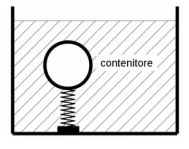
\includegraphics[scale=1.1]{ES4/GEN042018.jpg}
    \end{center}
\end{figure}